\documentclass[noraggedright]{turabian-researchpaper}

% Turabian Formatting
\usepackage{turabian-formatting}

% Chicago Bibliography Formatting
\usepackage[
  autocite = footnote,
  sorting=ynt,
  annotation]
  {biblatex-chicago}
   
\renewcommand{\bibfont}{\normalsize}
\addbibresource{Bibliography.bib}

% Language and Text Formatting
\usepackage[utf8]{inputenc}
\usepackage[T1]{fontenc}
\usepackage{microtype}
\usepackage[greek, english]{babel}
  \babeltags{en = english}
  \babeltags{el = greek}
\usepackage{teubner}

% Packages recommended for Turabian
\usepackage{threeparttable}
\usepackage{ellipsis}
\usepackage{tocloft}
\usepackage{csquotes}

% Title Page
\title{This Great Flood of Words\thanks{Rep. 1: 344 d1}}
\subtitle{A Brief Phasal Analysis of the Dialogue
  between Socrates and Thrasymachus}
\author{Thomas Broadwater}
\course{GREK 8010: Readings and Research in Greek Literature}
\submissioninfo{}
\date{\today}

\usepackage{Sweave}
\begin{document}
\Sconcordance{concordance:GreatFlood.tex:GreatFlood.Rnw:%
1 39 1 1 0 2 1 1 11 1 19 1 12 1 5 140 1 1 180 10 1 1 2 12 0 1 2 6 1 2 2 %
6 1 1 2 12 0 1 2 4 1 2 2 31 1 1 92 5 1 1 2 12 0 1 2 6 1 2 2 17 1 1 11 1 %
2 43 1}







\maketitle

\section{Goals and Methodology}
This study aims to establish a high-level phasal structure of the dialogue
between Socrates and Thrasymachus in Book 1 of Plato's Republic, as
translated by G.M.A. Grube and revised by C.D.C. Reeve. The elenctic style
of the argument presented in Plato's writing involves metatextual details as
much as the arguments themselves, using the characterization of the
interlocutors to position these individuals' stances relative to one another.
This sort of metatextual characterization is apparent in Thrasymachus' very
name: \textel{θρασύ-μαχ-ο-ς}: bold-in-battle.%
\autocite[s.v. \textel{θράσυς}, \textel{θάρσος}; cf. Ther. \textel{Θ\hαρρύμαϙ\hς})]{Brill}
A simple name-reading prepares the audience for the rough treatment to come.

Deeper characterizations abound. ``Give an answer yourself, and tell us what you
say the just is,'' Thrasymachus demands of Socrates. ``And don't tell me it's
the right, the beneficial, the profitable, the gainful or the advantageous, but
tell me clearly and exactly what you mean; for I won't accept such nonsense from
you.'' (336 c4-d3) He cannot resist mockery and derision even in his most
reasonable requests. Thrasymachus knows the correct answer — his correct answer
— and all else is so much nonsense.

Socrates, for his part, replies with his fateful sarcasm as Thrasymachus 
presses him for an answer. When Thrasymachus, gloating, accuses Socrates of
being deceitful (337 a3, a5) and claims to have foretold such an occasion,
Socrates cedes this conflict, but only with a barb meant to draw Thrasymachus
into the dialectic. ``That's because you're a clever fellow, Thrasymachus.''
(337 a7) One must, of course, never assume themselves clever around Socrates.

\vspace*{1\baselineskip}
\noindent There are means of deepening this sort of analysis. By examining
phrases and the specifics of their wording — the chosen vocabulary, word
arrangement, and length of sentence, among others —  emergent patterns are made
to reveal themselves. These patterns recontextualize the piece, demarcating
interwoven segments called phases.

The piece is framed as a direct quote from Socrates as he retells a
previous conversation and so includes occasional narrative asides meant to
guide the reader. These include shorter phrases such as ``he said'' and ``he
replied,'' as well as lengthier elements, such as the description of
Thrasymachus blushing. While certainly part of a higher-level discourse, they
impede any discourse analysis and so are removed from the data.The remaining 301
turns in the conversation make up the core data set.

Five individuals participate in this dialogue: Cleitophon, Glaucon, Polemarchus,
Socrates, and Thrasymachus. The speakers typically take turns speaking with
Socrates, but not exclusively. For example, there is a short digression between
Cleitophon and Polemarchus as they attempt to pin down the specific meaning of
Thrasymachus' stance on the nature of justice (340 a1 - 340 b9), which Socrates
quickly stops. Glaucon also enters the conversation at two points, once
addressing Thrasymachus in support of Socrates (337 d7 - d8) and later asking
Socrates for clarification on a point (347 a7 - 348 b6). These asides are brief
as a rule, but they are undeniably a part of the dialogue and are retained in
the data.

Whenever a sentence is quoted directly, it will be presented in a specific
notation from this point on. First will come the Stephanus Pagination. Second
will come a token specifying the speaker and the turn. For example, Glaucon's
first turn will have the token G1, his second G2. Third will come a letter
indicating the sentence in the turn. The first sentence will be
labeled a./, the second b./, and so on. Last will come the text. To exemplify,
Socrates' seventh turn in the conversation reads as follows.

\begin{quote}
\emph{337 d2-d4, S7} a./ What else than the appropriate penalty for one who doesn't
know, namely, to learn from the one who does know? b./ Therefore, that's what
I deserve.
\end{quote}

This study will use the programming language R to analyze three key markers:
the number of words in each turn, the number of sentences in each turn, and the
sentiment of each turn. This study uses G.M.A. Grube's and C.D.C. Reeve's
translation of the Republic, as mentioned above, to facilitate the use of
programmatic methods. To attempt this study on the Greek text would require
three significant undertakings.

First, the programmer would need to create a list of ``stop words.'' These are
short words that, while grammatically significant, are less semantically
relevant. The list would also need to be sensitive to context. For example,
the script may safely remove the particle ``\textel{δέ}'' from a great many
sentences, but removing it from a  ``\textel{ὁ μέν … ὁ δέ}'' construction would
remove important semantic material. The task would be of much greater scope
than this study.

Unlike Greek, typical English prose is less reliant on sentence particles, and
so a computer may remove stop words from a text with less trepidation. In
addition, the tools for removing English stop words already exist, and their
engineers have had years to solidify their lists. Taking advantage of these
preexisting tools clears the way for quicker and simpler analyses.

Second, the programmer would need to create a tool to derive the lemma form —
i.e., the dictionary form — of each word encountered. Computers cannot simply
identify such elements as verbal roots in the same way a person can, so some
method of disambiguating forms would be necessary. Without this tool, the
computer would have no understanding that different forms may be from the
same word. For example, the words ``\textel{ἔλυσα}'' and ``\textel{ἐλύθην}''
would read as completely distinct elements, ignoring the apparent relationship
between the two.

English again differs from Greek in this regard. Given that English lacks the
thorough conjugation and declension patterns found in Greek, an adequately
written program can derive English lemma forms much more easily. The R
community has also produced such tools side-by-side with stop word lists, making
them more immediately available and further simplifying the study.

Third, the programmer would need to create a sentiment dictionary for Ancient
Greek. A sentiment dictionary is a lexicon of the moods or feelings connoted by
the words it contains. The standard R libraries include four sentiment
dictionaries. The Bing and Loughran lexicons use a simple binary for their
definitions: positive-negative. For example, "prison" is marked as negative,
while ``free'' is marked as positive. The NRC lexicon attempts to define
specific emotions, such as ``trust,'' ``fear,'' and ``anger;'' as well as the
more ambiguous ``positive'' and ``negative.'' The AFINN lexicon strikes a
compromise between the binary approach of Bing and Loughran and the specific
definitions of NRC. Each word is placed on a sentiment range from -5 (most
negative sentiment) to +5 (most positive sentiment). The effort required to
replicate one of these dictionaries in Greek, a process that would rely on
preexisting stop word lists and lemmatizers, would be tremendous. Teams of
programmers typically undertake projects of this size, and the lack of options
should speak to the difficulty of their construction. 

This study will use the AFINN lexicon's sentiment range to identify transitions
in and out of phases. However, using the AFINN lexicon does require compromise.
Finn Årup Nielsen designed it for analyzing the sentiment of microblogs, and the
sentiment scores are specifically tailored for Twitter. Any sentiment analysis
undertaken will have a modern colloquial underpinning, and the analysis will
specifically represent a 21st-century reading of the text. Furthermore, the
lexicon excludes more words than are in the list of stop words used for this
study.

Consequently, the analysis output will necessarily be shorter than the input, 
ith gaps in the results. Despite this, the AFINN lexicon fits this study better
than the alternatives. The continuous range of scores offers more flexibility
than the binary options of the Bing and Loughran lexicons. The NRC lexicon,
while more specific, does not output a usable quantitative variable, whereas the
AFINN scores will readily function variables in statistical tests.

\section{Turn Density and Turn Length}



The first portion of the code tallies the number of sentences per turn, hoping to identify a correlation between turn ``density'' and the occurrence of phase transitions. It counts the data in two ways. First, it gathers ``global'' statistics, i.e., the relevant information from the entire dialogue, and second, it gathers speaker-by-speaker statistics. In order to construct a high-level view of turn density, the script returns a table of calculations. The \emph{mean} ($\bar{x}$) represents the average number of sentences per turn, and the \emph{standard deviation} ($\sigma$) represents the overall variation within the data. However, plain numbers describe little on their own. Therefore, the code also performs two statistical tests to help determine how meaningful the results are: a t-test and an F-test.

A t-test is a method for comparing two means against each other. The first mean is that of the \emph{population}: here, the interlocutors taken as a group. The population mean is the global mean described above. The second mean is that of the \emph{sample}: here, each speaker taken individually. The test returns a \emph{p-value}, which communicates the statistical significance of the difference between the means. To determine significance, the researcher compares a p-value against an \emph{α-value}, which they chose in advance. This study uses an α-value of 0.05, which is common in statistical research.

An F-test is similar to a t-test, but rather than comparing means, it compares \emph{variances} — i.e., standard deviations. The test uses the same population and sample population as a t-test and similarly returns a p-value. 

In both tests, if the p-value is lower than the α-value, then the differences are statistically significant. Both tests used in this study are two-tailed tests, meaning that they check if the sample statistic is either significantly larger or significantly smaller than the population statistic. Therefore, even if a p-value is lower than an α-value, there is no way to tell from the test alone if the sample statistic is significantly larger or smaller than the population statistic. To account for this, the t- and F-test results are included in the table of calculations. The column \texttt{p\_mean} contains the results of the t-tests, and the column \texttt{p\_sd} contains the results of the F-tests.

\begin{table}[htbp]
\begin{Schunk}
\begin{Soutput}
# A tibble: 6 × 5
  speaker      mean  p_mean    sd      p_sd
  <chr>       <dbl>   <dbl> <dbl>     <dbl>
1 global       1.69 NA      1.79  NA       
2 cleitophon   1.33  0.392  0.577  0.197   
3 glaucon      1.25  0.0300 0.463  0.000898
4 polemarchus  1.75  0.915  0.957  0.327   
5 socrates     1.99  0.0580 1.90   0.427   
6 thrasymacus  1.41  0.0538 1.72   0.591   
\end{Soutput}
\end{Schunk}
\caption{Turn Density Data}
\label{tab:DensityData}
\end{table}

The code also returns a bar chart of turn densities. The x-axis represents the turn, and the y-axis represents the density. The x-axis is labeled with each turn's index number, which designates the order in which they appear. For example, the index 94 (i94) corresponds to Thrasymachus' 44th turn (T44), the major outlier of the set.

\begin{figure}[htbp]
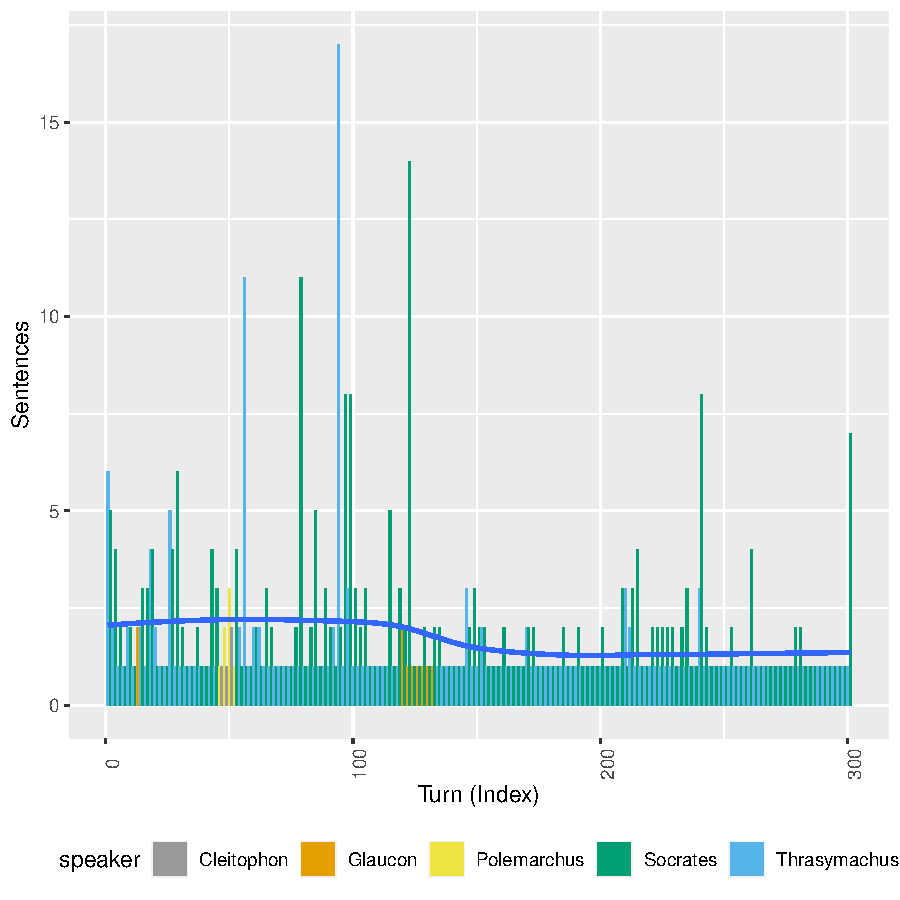
\includegraphics{GreatFlood-Figure: Turn Conseq}
\caption{Turn Density by Index}
\label{fig:DensityPlot}
\end{figure}

The second portion of the code tallies the number of words per turn, hoping to identify a correlation between turn ``length'' and the occurrence of phase transitions. Once again, it counts the global and speaker-by-speaker statistics, which it then uses as variables for t- and F-tests. The code also returns a bar chart of turn lengths. The x-axis represents the turn, and the y-axis represents the length.

\begin{table}[hbtp]
\begin{Schunk}
\begin{Soutput}
# A tibble: 6 × 5
  speaker      mean   p_mean    sd      p_sd
  <chr>       <dbl>    <dbl> <dbl>     <dbl>
1 global      25.5  NA       48.6  NA       
2 cleitophon  20     0.561   13.7   0.154   
3 glaucon      9.38  0.00253  9.94  0.000189
4 polemarchus 28.2   0.875   32.3   0.553   
5 socrates    36.4   0.00362 44.9   0.274   
6 thrasymacus 14.9   0.0178  52.1   0.322   
\end{Soutput}
\end{Schunk}
\caption{Turn Length Data}
\label{tab:LengthData}
\end{table}

\begin{figure}[htbp]
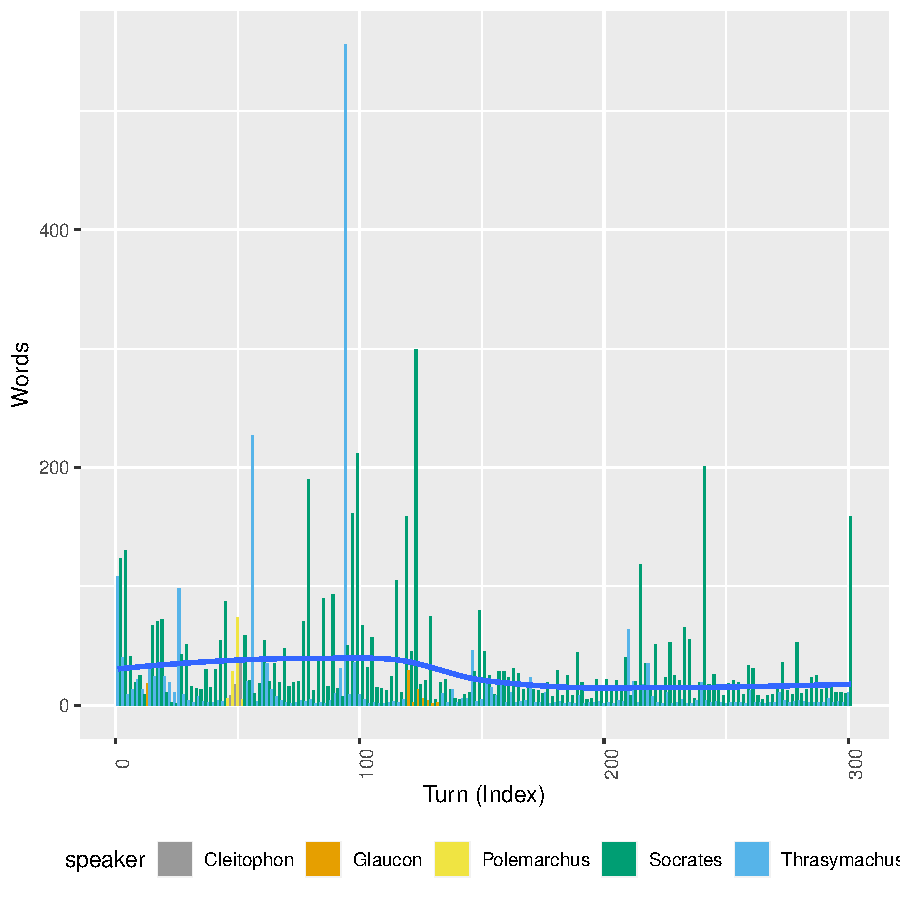
\includegraphics{GreatFlood-Figure: Turn Len}
\caption{Turn Length by Index}
\label{fig:LengthPlot}
\end{figure}

The results of these tests show a very regular data set. Turn density, in particular, is consistent across speakers, with means and standard deviations typically not differing significantly per speaker from the global. This regularity reflects the call-and-response nature of Plato's dialogues. However, Glaucon's means and standard deviations are significantly lower than the global with respect to both density and length. Glaucon frequently took shorter, less dense turns than the other interlocutors, representing his character's role in the dialogue.

Glaucon's character filled the role of a didactic tool, enabling Socrates to establish and elaborate on his arguments. In his first turn, 337 d7 - d8,
Glaucon enabled Socrates financially.

\begin{quote}
\emph{337 d5, T6} a./ You amuse me, but in addition to learning, you must pay a fine.\\
\emph{337 d6, S6} a./ I will as soon as I have some money.\\
\emph{337 d7-d8, G1} a./ He has some already[.] b./ If it's a matter of money, speak, Thrasymachus, for we'll all contribute for Socrates.\\
\emph{337 d9, T7} a./ I know[,] so that Socrates can carry on as usual.
\end{quote}

Glaucon's intervention allowed Socrates to carry on the conversation by removing any financial requirements imposed by Thrasymachus. This action established Glaucon as an auxiliary to Socrates, preparing the reader for his intervention in his second turn, 347 a7 - a9.

Thrasymachus has, by this point, argued that one rules if and only if they are acting to their own advantage and, by conflating advantage with the subjugation of the ruled, that it is in the nature of a ruler to act tyrannically. Socrates counters this with a demonstration that ruling benefits the rules in the same way that medicine benefits the sick and not the doctor. That, just as the doctor requires a wage, so too does the ruler require a wage in the form of money or honor. So, as he states in 346 e3 - 347 a6 (S58), the ruler is compelled by a wage to act for the benefit of the ruled. This statement is structured as a conclusion to the prior arguments, providing a natural opportunity to change turns — however, Socrates has a third point to make. He wants to argue that punishments also wages, from the mindset that punishments, like money and honor, are external motivators. Yet, at that moment, Thrasymachus had the opportunity to interject and change the course of the argument before this last point were made. 

\begin{quote}
\emph{346 e3 - 347 a6, S58} a./ Then, it is clear now, Thrasymachus, that no craft or rule provides for its own advantage, but, as we've been saying for some time, it provides and orders for its subject and aims at its advantage, that of the weaker, not the stronger. b./ That's why I said just now, Thrasymachus, that no one willingly chooses to rule and to take other people's troubles in hand and straighten them out, but each asks for wages; for anyone who intends to practice his craft well never does or orders what is best for himself — at least not when he orders as his craft prescribes — but what is best for his subject. c./ It is because of this, it seems, that wages must be provided to a person if he's willing to rule, whether in the form of money or honor or a penalty if he refuses.\\
\emph{347 a7-a9, G2} a./ What do you mean, Socrates[?] b./ I know the first two kinds of wages, but I don't understand what penalty you mean or how you can call it a wage.
\end{quote}

Glaucon capitalized on this turning point. He filled the open space and, in doing so, enabled Socrates to elaborate on his third point. In the following question-and-answer sequence between the two, Glaucon does nothing but affirm and agree, offering little of his own perspective. His character exclusively enabled Socrates to control the conversation and disappeared entirely from the dialogue when this role is complete. His role as a didactic tool, rather than an individual character in its own right, colored his dialogue, resulting in significantly shorter turns than the rest of his interlocutors.

\noindent Socrates and Thrasymachus both show significantly different means from the global but in different ways. Socrates' turns are, on average, significantly longer than the global. This difference is consistent with his role in the narrative. As the main character and the primary delivery method for philosophical ideas, Socrates needs more time than the other speakers to argue his positions thoroughly and precisely dissect the inconsistencies of opposing viewpoints. 

On the other hand, Thrasymachus shows significantly shorter turns than the global. This difference is also consistent with his role in the narrative. As the main antagonist of the dialogue, it is the role of Thrasymachus to deliver his assertions and seem them summarily decomposed. So then, his turns should be relatively short, as he makes way for Socrates to interrogate his positions.

\section{Sentiment Analysis}

The code proceeds to tally the average sentiment per turn, hoping to identify a correlation between turn sentiment and the occurrence of phase transitions. 

Once again, the code calculates the means and standard deviations of the whole text and the individual speakers, then tests the results for significants with t- and F-tests. The results are noteworthy: not a single speaker significantly differs from the global calculations. 

\begin{table}[hbtp]
\begin{Schunk}
\begin{Soutput}
# A tibble: 6 × 5
  speaker       mean p_mean    sd   p_sd
  <chr>        <dbl>  <dbl> <dbl>  <dbl>
1 global       0.415 NA      1.43 NA    
2 cleitophon   2     NA     NA    NA    
3 glaucon     -0.5    0.651  2.12  0.279
4 polemarchus  0.519  0.906  1.34  0.830
5 socrates     0.433  0.901  1.50  0.581
6 thrasymacus  0.380  0.840  1.30  0.417
\end{Soutput}
\end{Schunk}
\caption{Turn Sentiment Data}
\label{tab:SentimentData}
\end{table}

However, the data set returned by the command \texttt{get\_sentiments()} is shorter than the data set entered by a wide margin. The command removed 130 turns from the data set for a 43\% loss of turns. The gaps introduced by the analysis significantly reduce the usefulness of the results. A bar graph of the results is printed below.

\begin{figure}[htbp]
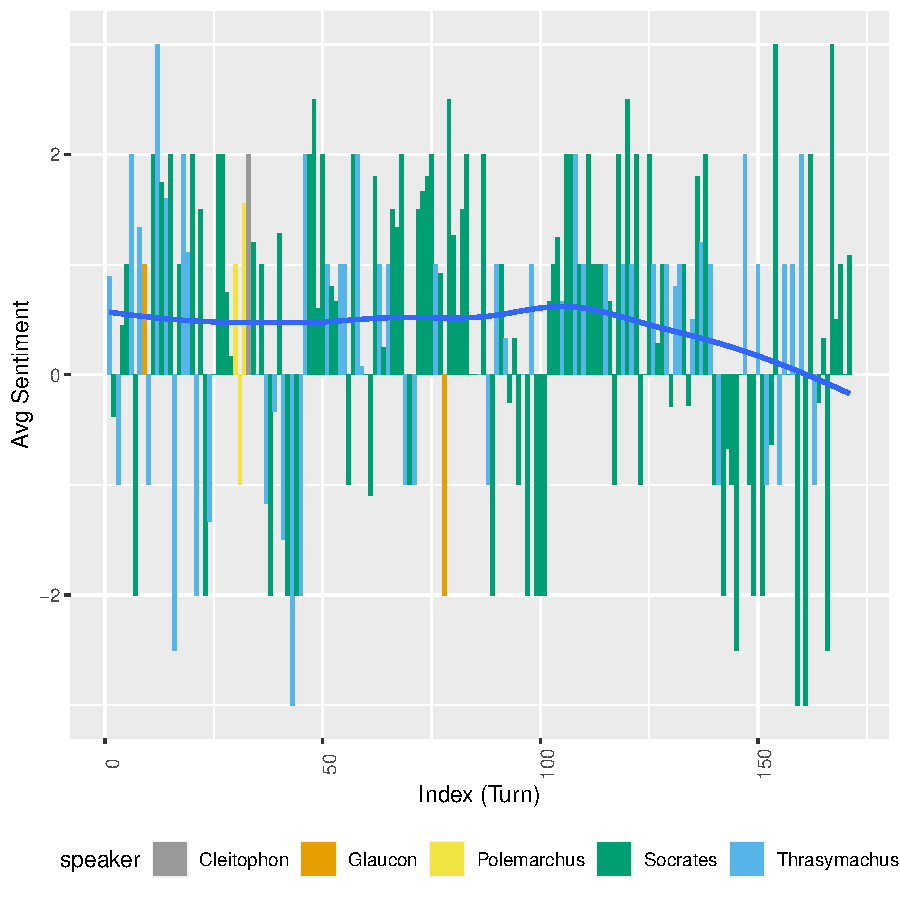
\includegraphics{GreatFlood-Figure: Turn Sen}
\caption{Average Sentiment by Index}
\label{fig:SenPlot}
\end{figure}

Without comparable tools to perform a sentiment analysis of the text in Greek, it is difficult to say where this even score comes from. The data may reflect an original attempt by Plato to give an even-handed treatment of all sides, but this seems inconsistent with Thrasymachus' introduction. His first turn, during which he is supposed to have ``hurled himself at [Socrates and Simonides] as if to tear [them] to pieces'' (336 b3-b4), has an average sentiment of +0.8 — middlingly positive. Thrasymachus' 44th turn, in which he openly advocates for despotic governance, has an average sentiment of +0.07 — explicitly neutral. 

Instead, the results reflect a fundamental difference between good academic prose and good colloquial prose. In the Classics, where ancient texts are commonplace or, for many, the study itself, the prose is expected to display a high proficiency in an academic style, retaining rules and structures inspired by prose in the classical languages. This specificity carries over to translations of classical texts. If the audience is already primed to accept and parse these features, then there is every incentive to remain faithful to the original texts. Moreover, the translator can expect the audience to understand the connotations of the text despite, or even owing to, these shared features.

Colloquial prose, which the Afinn lexicon was explicitly designed for, does not confine itself to the same priorities. For example, it is far more acceptable in colloquial prose to emphasize shades of meaning through competing vernacular terms and varying adherence to prescribed grammaticality than in academic prose, where such formations may read as incorrect. 

The results seem to suggest that the full connotative force of Thrasymachus' arguments is not expressed in such a way as to impact a broader audience significantly. Regardless of the translation's qualities as an academic-facing document, the sentiment analysis results may indicate a lack of approachability for the typical reader — an implication owed further investigation but outside the scope of this study.

\section{Analysis}
In figure 1 ``Turn Density by Index'' and in figure 2 ``Turn Length by Index'' there are corresponding downward turning points in the moving averages at roughly turn 125. After this point, the average turn densities and lengths remain low compared to their starting values for the rest of the discourse.

Focusing on the first 150 turns reveals a pattern in Thrasymachus' turn lengths. Starting at turn 18, Thrasymachus' turns are punctuated by long speeches followed by periods of short statements. The cycle starts at turn 18, then iterates at turns 26 and 56. With each long turn, the duration of the cycle increases. The first cycle lasts 8 turns, from the start of turn 18 to the end of 25; the second cycle lasts 30 turns, 26 to 55; the third cycle lasts 38 turns, from 56 to 93.

\begin{figure}[htbp]
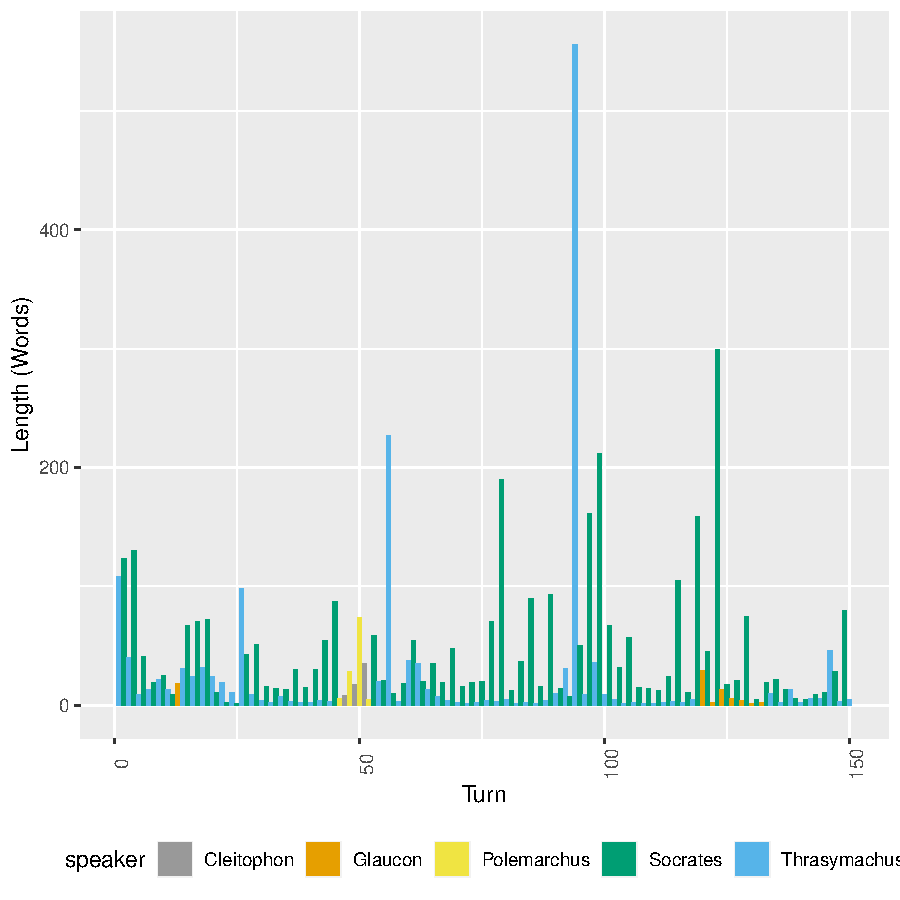
\includegraphics{GreatFlood-Fig: P1 Lengths}
\caption{Turns 1-150, Length by Index}
\label{Fig:P1Turns}
\end{figure}

Socrates' turns show an inverse pattern, though less uniform. As Thrasymachus' turns decrease in length, Socrates' generally increase, especially during the second and third cycle.

The cycles correspond to the stages of Thrasymachus' argument. At turn 18 – representing 338 c1 - c3, T9 – Thrasymachus proposes the softest version of his thesis: that justice is whatever serves the advantage of the stronger. Socrates tries to ask for clarification, but Thrasymachus, already frustrated, forces Socrates to answer his own questions. The interruption of Socrates' cycle is indicative of Thrasymachus' overbearance in the conversation.

At turn 26 – representing 338 d10 - 339 a3, T14 – Thrasymachus begins the second iteration of the cycle by reframing his argument to be about the relationship of a ruler to the ruled. After conflating the rulers of the state with the stronger, clarifying that he generally means the socially strong, not the physically strong, Socrates throws him off his rhythm by pointing out the hypocrisy of Thrasymachus' answer

\begin{quote}
\emph{339 a4-a7, S14} a./ Now I see what you mean. Whether it's true or not, I'll try to find out. b./ But you yourself have answered that. the just is the advantageous, Thrasymachus, whereas you forbade that answer to me. c./ True, you've added ``of the stronger'' to it.\\
\emph{339 b1, T15} a./ And I suppose you think that's an insignificant addition.\\
\emph{339 b2-b5, S15} a./ It isn't clear yet whether it's significant. b./ But it is clear that we must investigate to see whether or not it's true. c./ I agree that the just is some kind of advantage. d./ But you add that it's of the stronger. e./ I don't know about that. f./ We'll have to look into it.\\
\emph{339 b6, T16} a./ Go ahead and look.\\
\emph{339 b7, S16} a./ We will. b./[ ... ]
\end{quote}

Thrasymachus slips into sullen terseness as Socrates capitalizes on the new social opening offered in T16 with a new round of questions. Socrates enters his inverse pattern and wrestles the conversation away from Thrasymachus. The process is so complete that Cleitophon and Polemarchus enter the conversation near the end of this cycle's iteration. They speak to the exclusion of Thrasymachus, having their own debate over how they interpreted the intent of his statements until Socrates deliberately reintroduces him.

At turn 56 – 340 d10 - 341 a4, T25 – Thrasymachus begins the third iteration of the cycle with an attempt to regain control of the argument. His frustration becomes apparent as he resumes his insults. His failure to shift the course of the conversation is apparent in his terseness and angry outburst in turn 94 – 343 b1 - 344 e6, T44. This is the point where Thrasymachus presents the clearest version of his viewpoint: oppressive policies by despotic governments are examples of justice.

Socrates delivers relatively long turns for the next few moments, first admitting to being dumbstruck and then capitalizing on Glaucon's intervention to argue a minor point. This keeps the average density and length artificially high, but the mood changes visibly after Thrasymachus' speech. The data shows a steep decrease in turn densities and lengths, showing that whatever jovial mood remained was deflated. The interruptions from outsiders to the conversation also cease after this exchange, suggesting an unwillingness of the other party-goers to engage with the two main speakers. In other words, the figures show the moment when Thrasymachus ruins the party for everyone else.

This point also indicates a change in conversation as Socrates and Thrasymachus shift away from discussing the nature of justice and into whether justice is a vice or virtue. Given the shift in both pattern and topic of conversation, the outburst in T44 marks the end of the first phase ($P_1$). The outburst proper is the transition out of $P_1$, while Socrates' attempts to orient himself mark the transition into $P_2$.

Socrates, interestingly, mentions this topic change along with a change to the topic of profitability at the end of Book 1.

\begin{quote}
\emph{354 b3 - b7, S149} e./ Before finding the answer to our first inquiry about what justice is, I let that go and turned to investigate whether it is a kind of vice and ignorance or a kind of wisdom and virtue. f./ Then an argument came up about injustice being more profitable than justice, and I couldn't refrain from abandoning the previous one and following up on that.
\end{quote}

\noindent The paragraph functions like a soliloquy and seems a rather apparent insertion by Plato meant to conclude the argument so far. Plato mentioning both topic changes in a row may imply that the second is also indicative of a phase change, but this is inconsistent with the structure of the text. Rather than being an outright change, the second topic is buried in Socrates' aside with Glaucon and later returned to after Thrasymachus asserts justice to be a vice. Plato's insertion does not address this structure. It is fitting that Plato organized his conclusion this way since his goal seemingly was to touch on each central point in one small paragraph. It would have made for a confusing closing statement if he were to mirror the dialogue structure in his conclusion. However, it has the unintended effect of suggesting a phase change where one does not exist. The data gathered shows no discernable relationship between the second topic shift and turn measurements.

Of course, the downward turning point does not align perfectly with the first phase change, just as the upward turning point does not align perfectly with a hypothetical second. However, in the first case, the turning point was delayed by Glaucon handing Socrates a chance to speak at length without interruption. However, the second turning point does not have a comparable factor to explain why it preempts the reintroduction of the profitability topic. Instead, the turning point is indicative of the new pace of conversation maintained through Socrates' extended questioning of Thrasymachus.

\vspace*{1\baselineskip}
\noindent Overall, the data suggest a two-phase structure, pivoting around Thrasymachus' transition from an audience member to the main interlocutor positioned against Socrates. The first phase involves all five interlocutors, whereas the second barely includes Glaucon and is entirely devoid of both Polemarchus and Cleitophon. Furthermore, while the first phase is characterized by a relatively high average length and density of turn, the second is characterized by lower averages that increase subtly over time. The change between these two norms occurs during the transition into $P_2$. During this time, Socrates argues a minor point against Thrasymachus' position on the volition of rulers, briefly introduces the topic of profitability, and draws out Thrasymachus' stance on justice as a virtue. After this, Socrates returns to profitability, which remains the primary topic for the rest of the book, signaling the end of the transition and entering the main body of $P_2$.

\clearpage
\nocite{*}
\printbibliography[keyword={texts}]
\printbibliography[keyword={packages},title={Software}]
\end{document}
